\section{Lektion 13-03-2018}

\begin{enumerate}
	\item Transistorer
	\item Y-parametre
	\item Toporte
	\item Stabilitet
	\item Input- output admittancer
\end{enumerate}

\begin{mdframed}[style=exampledefault]
	\begin{itemize}
		\item \textbf{Pensum:} CB, Ch 5 p. 103-123, Ch 6 p. 125-131
		\item \textbf{Opgaver:} Lektion 5-1
	\end{itemize}
\end{mdframed}

\subsection{Transistorer}
\subsubsection{Typer}
\begin{itemize}
	\item Bipolar Junction Transistors (BJTs) or simply bipolars.
	\item Field Effect Transistors (FETs). 
	\begin{itemize}
		\item Bipolars have abrupt junctions in the semiconductor material and
		FET's do not.
		\item FETs have a gate element that creates an electromagnetic field when charged.
		\begin{itemize}
			\item FET's are voltage-controlled (gate charged).
			\item BJT's are current controlled (small current flowing).
		\end{itemize}
	\end{itemize}
\end{itemize}

\subsubsection{Semiconductor materialer}
\begin{itemize}
	\item Lateral-Diffused (LD) MOSFET's
	\item Gallium-Arsenide (GaAs) metal-semiconductor FET's (MESFET's)
	\item GaAs/InGaP heterojunction	bipolar transistors (HBT's)
	\item Gallium-Nitride (GaN)	high-electron-mobility transistors (HEMT's)
	\item Silicon-Carbide (SiC) FET's
\end{itemize}

\begin{figure} [H]
	\centering
	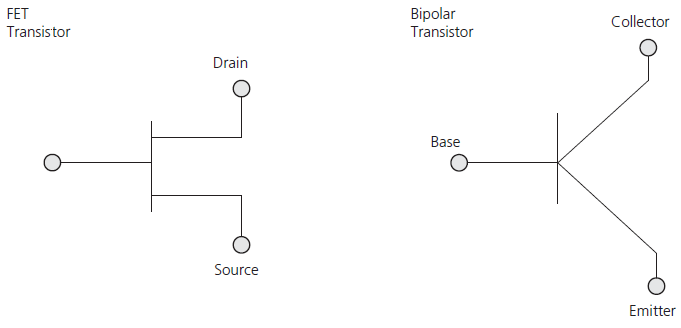
\includegraphics[width=0.8\linewidth]{graphics/31.png}
	\caption{FET and BJT.}
	\label{fig:31}
\end{figure}

\subsubsection{Model (Transistor equivalent circuit)}
At high frequencies, it's important to include package parasitics in design!

\begin{figure} [H]
	\centering
	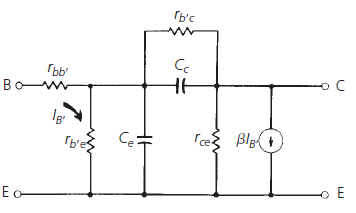
\includegraphics[width=0.6\linewidth]{graphics/32.png}
	\caption{Transistor equivalent circuit.}
	\label{fig:32}
\end{figure}

\begin{figure} [H]
	\centering
	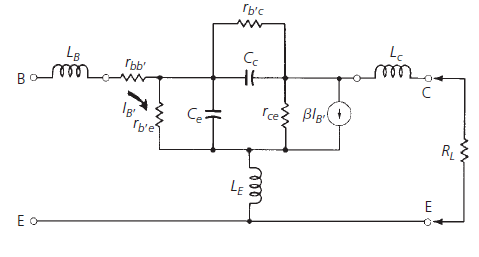
\includegraphics[width=0.8\linewidth]{graphics/33.png}
	\caption{Transistor equivalent circuit with lead inductance.}
	\label{fig:33}
\end{figure}

\begin{itemize}
	\item $r_{bb'}$ Base spreading resistance
	\item $r_{b'e}$ Input resistance
	\item $r_{b'c}$ Feedback resistance
	\item $r_{ce}$ Output resistance
	\item $C_e$ Emitter diffusion capacitance
	\item $C_c$ Feedback capacitance
	\item $\beta I_{B'}$ Current source
\end{itemize}

\subsubsection{Input impedance}
\begin{itemize}
	\item First simplification to the circuit of is to eliminate $r_{b'c}$.
	\item Secound simplification is to use the Miller effect to transpose
	$C_c$ from its series base-to-collector connection to be parallel with $C_e$.
	\begin{itemize}
		\item A new total capacitance of $C_T$.
	\end{itemize}
\end{itemize}

\begin{equation}
Z_{in} = j\omega L_B + r_{bb'}+\dfrac{\frac{1}{j\omega C_T}(r_{b'e})}{\frac{1}{j\omega C_T+r_{b'e}}}+j\omega L_E
\end{equation}

\begin{equation}
Z_{in} = j\omega (L_B+L_E) + r_{bb'}+\dfrac{r_{b'e}}{1+r_{b'e}j\omega C_T}
\end{equation}

\begin{equation}
Z_{in} = j\omega L_T + r_{bb'}+\dfrac{r_{b'e}}{1+j\omega r_{b'e} C_T}
\end{equation}

\begin{figure} [H]
	\centering
	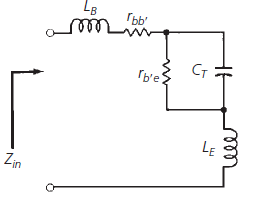
\includegraphics[width=0.4\linewidth]{graphics/34.png}
	\caption{Equivalent input impedance.}
	\label{fig:34}
\end{figure}

\subsubsection{Output impedance}

\begin{itemize}
	\item $r_{ce}$ and $r_{b'c}$ is very large in comparison to the other components and can usually be ignored.
	\item Changes in an external source resistance $R_s$ will also change $Z_{out}$.
\end{itemize}

\begin{figure} [H]
	\centering
	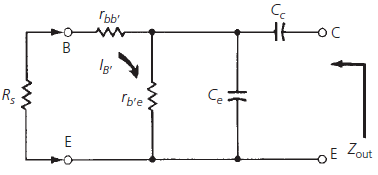
\includegraphics[width=0.6\linewidth]{graphics/35.png}
	\caption{Equivalent output impedance.}
	\label{fig:35}
\end{figure}


\subsection{Y-parametre}
\begin{itemize}
	\item Admittance is the reciprocal of impedance.
	\item It is expressed in the form of $Y =G\pm jB$
	\begin{itemize}
		\item G is conductance or the reciprocal of resistance.
		\item B is susceptance or the reciprocal of reactance.
	\end{itemize} 
	\item Characteristics at a certain frequency and bias point.
	\item Admittance parameters can be used to:
	\begin{itemize}
		\item Design impedance-matching networks for the transistor.
		\item Determine the transistors maximum available gain.
		\item Determine the transistors stability.
	\end{itemize}
\end{itemize}

\begin{figure} [H]
	\centering
	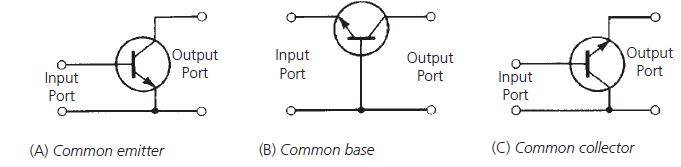
\includegraphics[width=\linewidth]{graphics/36.png}
	\caption{Three-terminal transistor as a two-port network.}
	\label{fig:36}
\end{figure}

\subsubsection{Toporte}

\begin{itemize}
	\item Black-Box configuration for the Y-parameter characterization.
	\item Short circuit used to make V1 and V2 equal to zero.
\end{itemize}

\begin{figure} [H]
	\centering
	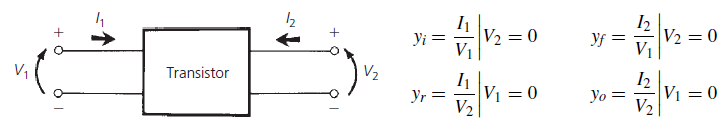
\includegraphics[width=\linewidth]{graphics/37.png}
	\caption{Short-circuit Y parameters.}
	\label{fig:37}
\end{figure}

\begin{itemize}
	\item $y_i = y_{11}$ short-circuit input admittance
	\item $y_r = y_{12}$ short-circuit reverse-transfer admittance
	\item $y_f = y_{21}$ short-circuit forward-transfer admittance
	\item $y_o = y_{22}$ short-circuit output admittance
\end{itemize}

\begin{equation}
I_1 = y_{11} V_1 + y_{12} V_2
\end{equation}

\begin{equation}
I_2 = y_{21} V_1 + y_{22} V_2
\end{equation}

\begin{figure} [H]
	\centering
	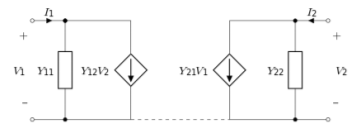
\includegraphics[width=0.6\linewidth]{graphics/38.png}
	\caption{Equivalent circuit for Y-parameters.}
	\label{fig:38}
\end{figure}

\subsection{S-parametre}
\begin{figure} [H]
	\centering
	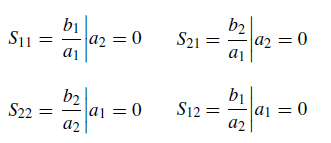
\includegraphics[width=0.5\linewidth]{graphics/40.png}
\end{figure}

\begin{equation}
b_1 = S_{11} a_1 + S_{12} a_2
\end{equation}

\begin{equation}
b_2 = S_{21} a_1 + S_{22} a_2
\end{equation}

\begin{itemize}
	\item $S_{11}$ input reflection coefficient
	\item $S_{12}$ reverse transmission coefficient
	\item $S_{21}$ forward transmission coefficient
	\item $S_{22}$ output reflection coefficient
\end{itemize}



\subsubsection{Conversion between Y and S}
\begin{figure} [H]
	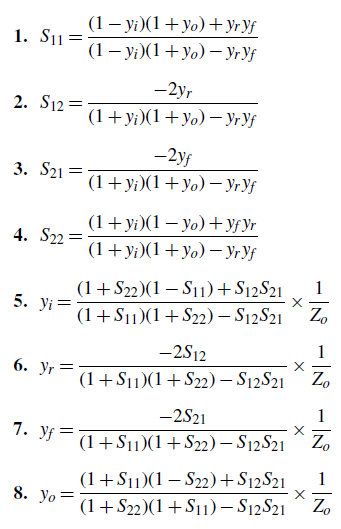
\includegraphics[width=0.5\linewidth]{graphics/39.png}
\end{figure}

\subsection{Stabilitet}
\subsubsection{Linvill stability factor}
\begin{itemize}
	\item $C < 1$ Unconditionally stable
	\item $C > 1$ Potentially unstable
\end{itemize}

\begin{equation}
C = \dfrac{|y_{12}y_{21}|}{2g_ig_o-Re(y_{12}y_{21})}
\end{equation}

\begin{itemize}
	\item $g_i$ input conductance
	\item $g_o$ output conductance
\end{itemize}

\subsubsection{Stern stability factor}
\begin{itemize}
	\item $K > 1$ Stable
	\item $K < 1$ Unstable
\end{itemize}

\begin{equation}
C = \dfrac{2(g_i+G_S)(g_o+G_L)}{|y_{12}y_{21}|+Re(y_{12}y_{21})}
\end{equation}

\begin{itemize}
	\item $G_S$ source conductance
	\item $G_L$ load conductance
\end{itemize}

\subsection{Maximum Available Gain}

\begin{equation}
MAG = \dfrac{|y_{21}|^2}{4g_ig_o}
\end{equation}